
\begin{frame}{Memory Referee}
\begin{itemize}
    \item Interface between multiple cores and the memory
    \item Forwards single petitions to the memory
    \item Controls the halt of the cores trying to access memory
    \item Scalable to any number of cores
\end{itemize}
\begin{figure}
    \centering
    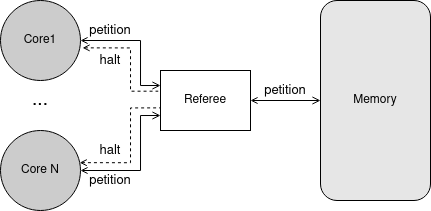
\includegraphics[width=6cm]{images/Referee_fig.png}
    %\caption{Caption}
    \label{fig:my_label}
\end{figure}
\end{frame}

% \begin{frame}{Memory Referee: Ports}
%   \begin{columns}[T]
%     \begin{column}{0.5\textwidth}
%     \textbf{Inputs:}\\
%         From cores:
%         \begin{itemize}
%             \item WR[ncores][1]
%             \item RD[ncores][1]
%             \item DADDR[ncores][32]
%             \item ST\_DATA[ncores][32]
%             \item BE[ncores][4]
%         \end{itemize}
%         From the memory
%         \begin{itemize}
%             \item MEM\_READY[1]
%             \item MEM\_VALID[1]
%             \item MEM\_LD\_DATA[32]
%         \end{itemize}
%     \end{column}
%     \begin{column}{0.5\textwidth}
%     \textbf{Outputs:}\\
%     To the cores
%     \begin{itemize}
%         \item HLT[ncores][1]
%         \item LD\_DATA[1]
%     \end{itemize}
%     To the memory
%     \begin{itemize}
%             \item M\_WR[1]
%             \item M\_RD[1]
%             \item M\_DADDR[32]
%             \item M\_ST\_DATA[32]
%             \item M\_BE[4]
%     \end{itemize}
%   
%     \end{column}
%  \end{columns}
% \end{frame}


\begin{frame}{Memory Referee: Behaviour}
  At any point:
  \begin{itemize}
      \item $PETITION[0..n]$ $\longleftarrow$ $RD[0..n]$ \hspace{0.2cm}$\mid$\hspace{0.2cm} $WR[0..n]$
      
      
      \item $HLT[0..n]$ $\longleftarrow$  $PETITION[0..n]$ \hspace{0.2cm}\&\hspace{0.2cm} $!RELEASE[0..n]$
  \end{itemize}
  
  \begin{columns}[T]
    \begin{column}{0.33\textwidth}
      \textbf{IDLE:}\\
      if $p>0$ petitions from the cores occur:
      \begin{enumerate}
          \item Select one $p_i$.
          \item Send $p_i$ to the main memory.
          \item Transition into WAITING.
      \end{enumerate}
    \end{column}
    \begin{column}{0.33\textwidth}
      \textbf{WAITING:}\\
      %Ignore all petitions.\\
      if $mem.valid==1$:
      \begin{enumerate}
          \item $RELEASE[i]=1$
          \item Transition into WAIT\_CORE
      \end{enumerate}
    \end{column}
    \begin{column}{0.33\textwidth}
      \textbf{WAIT\_CORE:}\\
      %Ignore all petitions.
      \begin{enumerate}
          \item $RELEASE[i]=0$
          \item Transition into IDLE
      \end{enumerate}
    \end{column}
  \end{columns}
\end{frame}

\begin{frame}{How to test it}
\begin{columns}[T]
    \begin{column}{0.4\textwidth}
	\textbf{Assembly inline}
    \end{column}
    \begin{column}{0.3\textwidth}
	\textbf{OBJDUMP}
    \end{column}
    \begin{column}{0.1\textwidth}
	\textbf{Hexfile}
    \end{column}
\end{columns}
\vspace{-0.5cm}
\begin{figure}
    \centering
    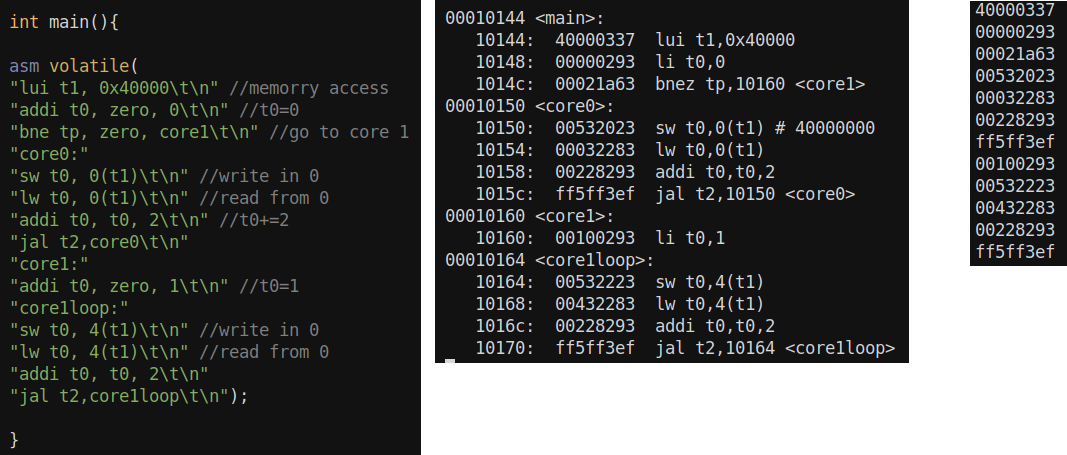
\includegraphics[width=11cm]{images/coding.png}
    %\caption{Caption}
    \label{fig:my_label}
\end{figure}


\end{frame}


\begin{frame}{FLAG test with two cores}
leds=[0 0 0 0], flag0=0, flag1=0.
  \begin{columns}[T]
    \begin{column}{0.4\textwidth}
        \textbf{Core0}\\
        while(1)\{\\
        \hspace{1cm}leds = [0 0 0 1];\\
        \hspace{1cm}flag0 = 1;\\
        \hspace{1cm}while(!flag1);\\
        \hspace{1cm}flag1 = 0;\\
        \hspace{1cm}leds = [0 1 0 0];\\
        \}
    \end{column}
    \begin{column}{0.4\textwidth}
        \textbf{Core1}\\
        while(1)\{\\
        \hspace{1cm}while(!flag0);\\
        \hspace{1cm}flag0 = 0;\\
        \hspace{1cm}leds = [0 0 1 0];\\
        \hspace{1cm}flag1 = 1;\\
        \}
    \end{column}
 \end{columns}
 \begin{figure}
    \centering
    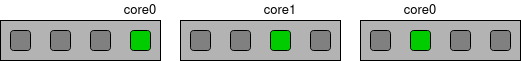
\includegraphics[width=8cm]{images/leds2_fig.png}
    %\caption{Caption}
    \label{fig:my_label}
\end{figure}
\end{frame}

\begin{frame}{FLAG test with two cores: Simulation}
\begin{figure}
    \centering
    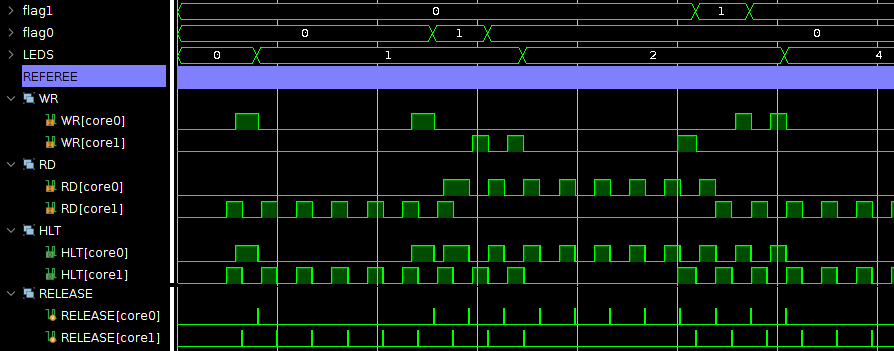
\includegraphics[width=11cm]{images/flag2_sim_crop.png}
    %\caption{Caption}
    \label{fig:my_label}
\end{figure}
\end{frame}

\begin{frame}{FLAG test with two cores: Simulation}
\begin{figure}
    \centering
    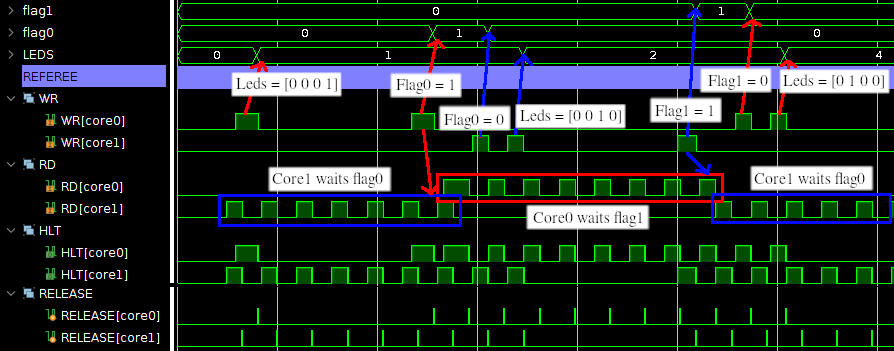
\includegraphics[width=11cm]{images/flag2_sim_crop_arrows.png}
    %\caption{Caption}
    \label{fig:my_label}
\end{figure}
\end{frame}

% \begin{frame}{FLAG test with two cores: Simulation}
% \begin{figure}
%     \centering
%     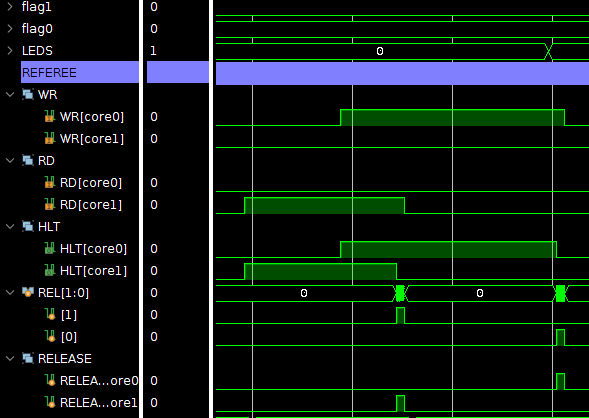
\includegraphics[width=8cm]{images/flag2_sim_close.png}
%     %\caption{Caption}
%     \label{fig:my_label2}
% \end{figure}
% \end{frame}

\begin{frame}{FLAG test with two cores: Simulation}
\begin{figure}
    \centering
    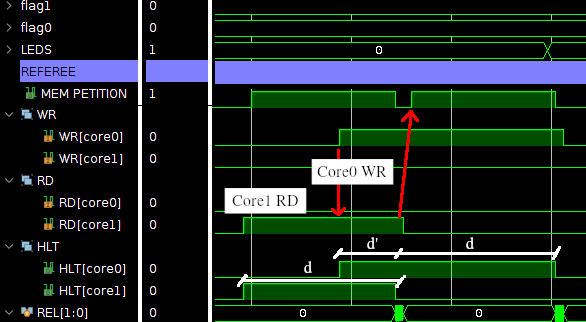
\includegraphics[width=8cm]{images/flag2_sim_close_arrow.png}
    %\caption{Caption}
    \label{fig:my_label2}
\end{figure}
\end{frame}

\begin{frame}{FLAG test with four cores}
  leds=[0 0 0 0], flag=0.
  \begin{columns}[T]
    \begin{column}{0.25\textwidth}
    \textbf{Core0}\\
    while(flag!=0);\\
    leds = [0 0 0 1];\\
    flag = 1;\\
    \end{column}
    \begin{column}{0.25\textwidth}
    \textbf{Core1}\\
    while(flag!=1);\\
    leds = [0 0 1 0];\\
    flag = 2;\\
    \end{column}
    \begin{column}{0.25\textwidth}
    \textbf{Core2}\\
    while(flag!=2);\\
    leds = [0 1 0 0];\\
    flag = 4;\\
    \end{column}
    \begin{column}{0.25\textwidth}
    \textbf{Core3}\\
    while(flag!=4);\\
    leds = [1 0 0 0];\\
    flag = 0;\\
    \end{column}
 \end{columns}
  \begin{figure}
    \centering
    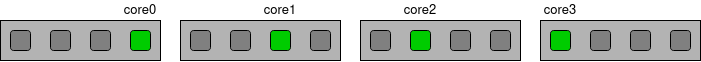
\includegraphics[width=10cm]{images/leds4_fig.png}
    %\caption{Caption}
    \label{fig:my_label}
\end{figure}
\end{frame}

\begin{frame}{FLAG test with four cores: Simulation}
\begin{figure}
    \centering
    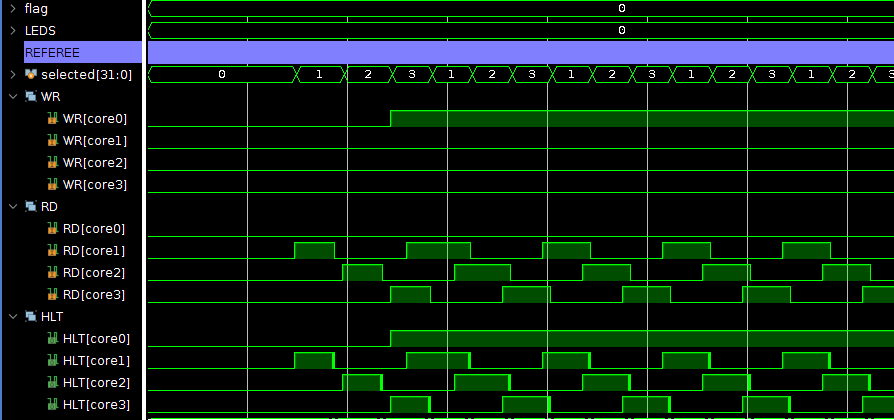
\includegraphics[width=11cm]{images/flag4_sim_bad_crop.png}
    %\caption{Caption}
    \label{fig:my_label}
\end{figure}
\end{frame}

\begin{frame}{FLAG test with four cores: Simulation}
\begin{figure}
    \centering
    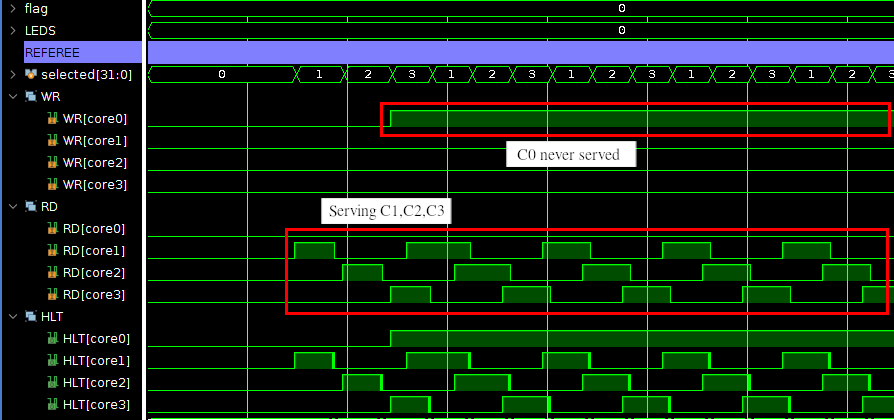
\includegraphics[width=11cm]{images/flag4_sim_bad_crop_arrow.png}
    %\caption{Caption}
    \label{fig:my_label}
\end{figure}
\end{frame}

\begin{frame}{FLAG test with four cores: Simulation}
\begin{figure}
    \centering
    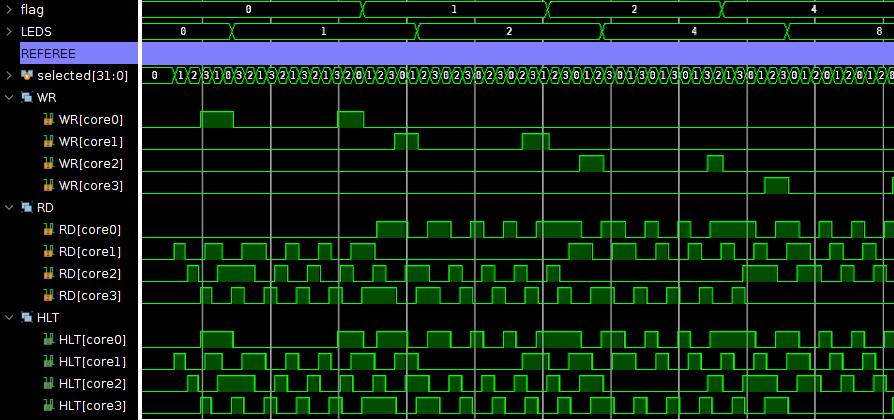
\includegraphics[width=11cm]{images/flag4_sim_good_crop.png}
    %\caption{Caption}
    \label{fig:my_label}
\end{figure}
\end{frame}

\begin{frame}{Axpy multicore}
axpy: $\sum_{i=0}^{n}{v_{i} * u_{i}}$
\vspace{0.2cm}
\begin{enumerate}
    \item Barrier after initialization
\end{enumerate}
\begin{figure}
    \centering
    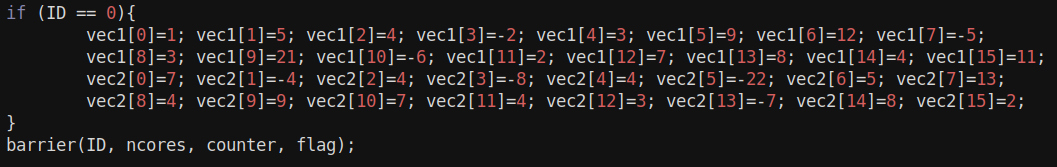
\includegraphics[width=11cm]{images/axpy_ini.png}
    \label{fig:my_label}
\end{figure}

\begin{enumerate}
    \item Reduction of the result
\end{enumerate}
\begin{figure}
    \centering
    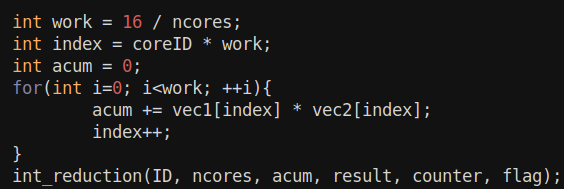
\includegraphics[width=6cm]{images/axpy_body.png}
    \label{fig:my_label}
\end{figure}


\end{frame}

\begin{frame}{Axpy with 4 cores: Simulation}
\begin{figure}
    \centering
    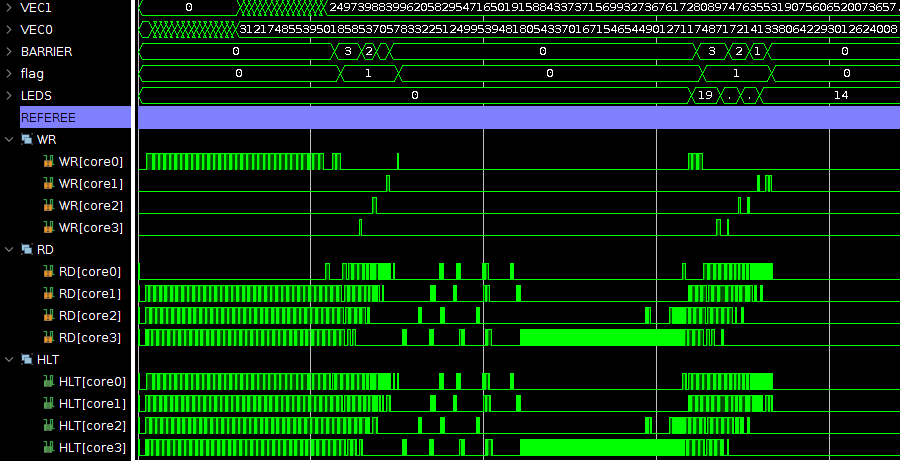
\includegraphics[width=11cm]{images/axpy_sim4_crop.png}
    %\caption{Caption}
    \label{fig:my_label}
\end{figure}
\end{frame}

\begin{frame}{Axpy with 4 cores: Simulation}
\begin{figure}
    \centering
    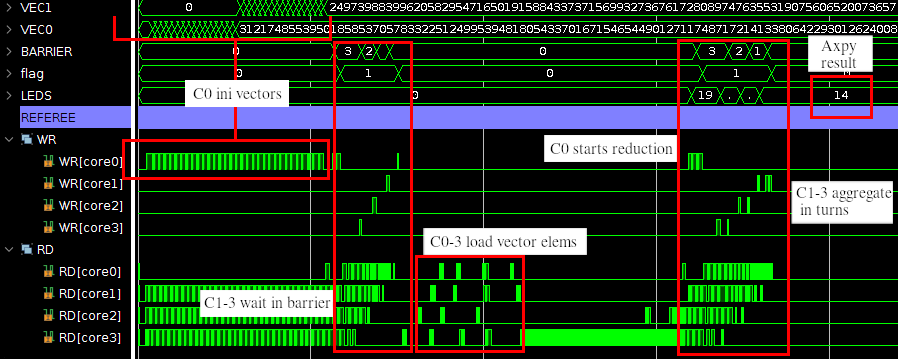
\includegraphics[width=11cm]{images/axpy_sim4_crop_arrow.png}
    %\caption{Caption}
    \label{fig:my_label}
\end{figure}
\end{frame}

\begin{frame}{Axpy with 8 cores: Simulation}
\begin{figure}
    \centering
    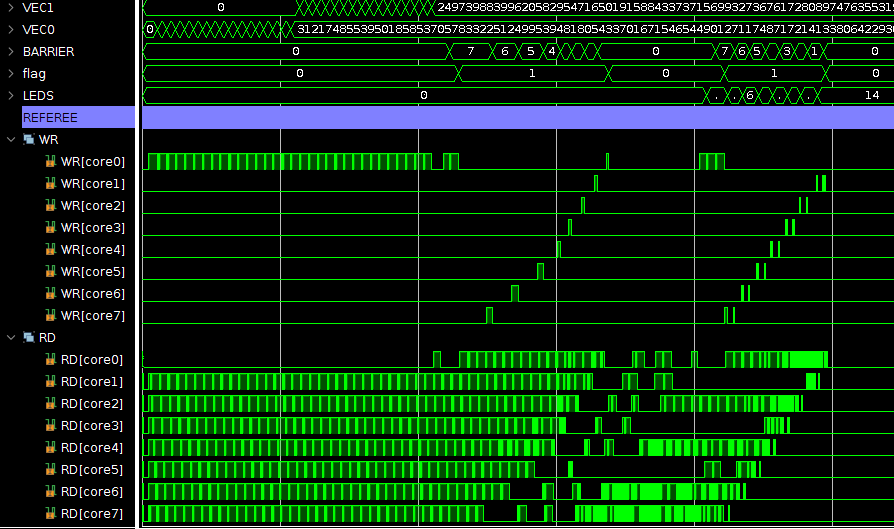
\includegraphics[width=11cm]{images/axpy_sim8_crop.png}
    %\caption{Caption}
    \label{fig:my_label}
\end{figure}
\end{frame}
